% Hlavicka pro protokoly z fyzikalniho praktika.
% Verze pro: LaTeX
% Verze hlavicky: 22. 2. 2007
% Autor: Ustav fyziky kondenzovanych latek
% Ke stazeni: www.physics.muni.cz/ufkl/Vyuka/
% Licence: volne k pouziti, nejlepe k vcasnemu odevzdani protokolu z Vaseho mereni.

\documentclass[a4paper,11pt]{article}

% Kodovani (cestiny) v dokumentu: utf-8
%\usepackage[cp1250]{inputenc}	% Omezena stredoevropska kodova stranka, pouze MSW.
\usepackage[utf8]{inputenc}	% Doporucujeme pouzivat UTF-8 (unicode).

%%% Nemente:
\usepackage[margin=2cm]{geometry}
\newtoks\jmenopraktika \newtoks\jmeno \newtoks\datum
\newtoks\obor \newtoks\skupina \newtoks\rocnik \newtoks\semestr
\newtoks\cisloulohy \newtoks\jmenoulohy
\newtoks\tlak \newtoks\teplota \newtoks\vlhkost
\usepackage{amsmath}
\usepackage{mathtools}
\usepackage{graphicx}
\usepackage{multirow}
\graphicspath{ {./images/} }
%%% Nemente - konec.


%%%%%%%%%%% Doplnte pozadovane polozky:

\jmenopraktika={Fyzikální praktikum 2}  % nahradte jmenem vaseho predmetu
\jmeno={Artem Gorodilov}            % nahradte jmenem mericiho
\datum={7. ~prosince  2023}        % nahradte datem mereni ulohy
\obor={Astrofyzika}                     % nahradte zkratkou vami studovaneho oboru
\skupina={Čt 8:00}            % nahradte dobou vyuky vasi seminarni skupiny
\rocnik={II}                  % nahradte rocnikem, ve kterem studujete
\semestr={I}                 % nahradte semestrem, ve kterem studujete

\cisloulohy={12}               % nahradte cislem merene ulohy
\jmenoulohy={Spektrometrické metody} % nahradte jmenem merene ulohy

\tlak={980}                   % nahradte tlakem pri mereni (v hPa)
\teplota={20.2}               % nahradte teplotou pri mereni (ve stupnich Celsia)
\vlhkost={41}               % nahradte vlhkosti vzduchu pri mereni (v %)

%%%%%%%%%%% Konec pozadovanych polozek.


%%%%%%%%%%% Uzitecne balicky:
\usepackage[czech]{babel}
\usepackage{graphicx}
\usepackage{amsmath}
\usepackage{xspace}
\usepackage{url}
\usepackage{indentfirst}
\usepackage{listings}
\usepackage{subcaption}
\usepackage{caption}
\usepackage{tabularx}
\usepackage[labelformat=parens,labelsep=quad,skip=3pt]{caption}

%%%%%% Zamezeni parchantu:
\widowpenalty 10000 \clubpenalty 10000 \displaywidowpenalty 10000
%%%%%% Parametry pro moznost vsazeni vetsiho poctu obrazku na stranku
\setcounter{topnumber}{3}	  % max. pocet floatu nahore (specifikace t)
\setcounter{bottomnumber}{3}	  % max. pocet floatu dole (specifikace b)
\setcounter{totalnumber}{6}	  % max. pocet floatu na strance celkem
\renewcommand\topfraction{0.9}	  % max podil stranky pro floaty nahore
\renewcommand\bottomfraction{0.9} % max podil stranky pro floaty dole
\renewcommand\textfraction{0.1}	  % min podil stranky, ktery musi obsahovat text
\intextsep=8mm \textfloatsep=8mm  %\intextsep pro ulozeni [h] floatu a \textfloatsep pro [b] or [t]

% Tecky za cisly sekci:
\renewcommand{\thesection}{\arabic{section}.}
\renewcommand{\thesubsection}{\thesection\arabic{subsection}.}
% Jednopismenna mezera mezi cislem a nazvem kapitoly:
\makeatletter \def\@seccntformat#1{\csname the#1\endcsname\hspace{1ex}} \makeatother

\begin{document}

\thispagestyle{empty}

{
\begin{center}
\sf 
{\Large Ústav fyzikální elektroniky PřF MU} \\
\bigskip
{\huge \bfseries FYZIKÁLNÍ PRAKTIKUM} \\
\bigskip
{\Large \the\jmenopraktika}
\end{center}

\bigskip

\sf
\noindent
\setlength{\arrayrulewidth}{1pt}
\begin{tabular*}{\textwidth}{@{\extracolsep{\fill}} l l}
\large {\bfseries Zpracoval:}  \the\jmeno & \large  {\bfseries Naměřeno:} \the\datum\\[2mm]
\large  {\bfseries Obor:} \the\obor  \hspace{40mm}  {\bfseries Skupina:} \the\skupina %
%{\bfseries Ročník:} \the\rocnik \hspace{5mm} {\bfseries Semestr:} \the\semestr  
&\large {\bfseries Testováno:}\\
\\
\hline
\end{tabular*}
}

\bigskip

{
\sf
\noindent \begin{tabular}{p{3cm} p{0.6\textwidth}}
\Large  Úloha č. {\bfseries \the\cisloulohy:} \par
\smallskip
$T=\the\teplota$~$^\circ$C \par
$p=\the\tlak$~hPa \par
$\varphi=\the\vlhkost$~\%
&\Large \bfseries \the\jmenoulohy  \\[2mm]
\end{tabular}
}

\vskip1cm
    \begin{minipage}[t]{0.5\textwidth} 
        \section{Zadání}
            Změřit koeficient propustnosti skla a fólie.
            \par Určit spektrální závislost indexu lomu. 
            \par Vypočítat tloušťku vrstvyz naměřené propustnosti. 
            \par Změřit absorpční koeficient pomocí Lambert-Beerova zákona.
        \section{Teorie}
            \subsection{Měření spektrální propustnosti}
                Při interakci světelné vlny s hranicí dvou prostředí se část její energie odrazí, zatímco druhá část přejde do dalšího prostředí. V druhém prostředí dochází k částečné absorpci světelné energie, zejména pokud je tloušťka prostředí malá. V případě, že k absorpci nedojde, zbývající energie po odrazu od druhé hranice látku opustí. Situaci lze vidět na obrázku (1).
                \par V optice existují tři charakteristiky popisující interakci světla se zkoumaným materiálem: odrazivost $R$, propustnost $T$ a absorpční koeficient $A$. Lze je zjistit pomocí následujících vzorců: 
                \begin{equation}
                    R = \frac{I_r}{I_0} 
                \end{equation}
                \begin{equation}
                    T = \frac{I_t}{I_0}
                \end{equation}
                Podle zákona zachování energie:
                \begin{equation}
                    R + T + A = 1
                \end{equation}
    \end{minipage}
    \hspace{10pt}
    \begin{minipage}[t]{0.5\textwidth} 
                \vspace{0pt}   
                \par \centering
                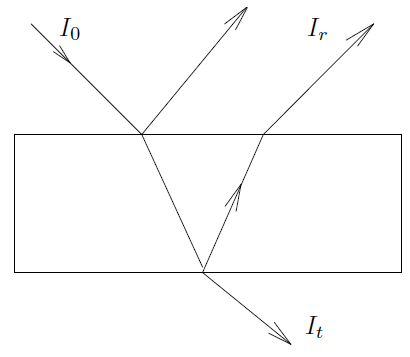
\includegraphics[scale=0.5]{int}
                \captionsetup{justification=centering, font=footnotesize}
                \captionof{figure}{$I_0$ intenzita dopadajícího světla, $I_r$ intenzita odraženého světla a $I_t$ intenzita světla procházejícího látkou.}
                \label{fig:int}
                \vspace{10pt}
                \raggedright
                \par K určení indexu lomu $n$ z propustnosti $T$ použijeme následující vzorec: 
                \begin{equation}
                    n = \frac{1+\sqrt{1 - T}}{T}
                \end{equation}
                Pro zjištění tloušťky materiálu je nutné zjistit jeho index lomu $n_{\nu}$ podle následujícího vzorce: 
                \begin{equation}
                    n_{\nu} = \frac{1+\sqrt{1 - T^{min}_f}}{T^{min}_f} \sqrt{n_s}
                \end{equation}
                kde $n_s$ je index lomu materiálu a $T^{min}_f$ se zjistí z níže uvedeného vzorce: 
                \begin{equation}
                    T^{min}_f = T_m \frac{1-R_s}{1+R_s (1-T_m)}
                \end{equation}
                kde $T_m$ je propustnost v lokálním minimu funkce propustnosti v závislosti na vlnové délce $\lambda$.
    \end{minipage}
\newpage
    \begin{minipage}[t]{0.5\textwidth} 
                Kde pro veličiny $T_m$ a $R_s$ platí vztahy:
                \begin{equation}
                    T_m = \frac{T_{fs}}{T_{ss}}
                \end{equation}
                kde $T_{ss}$ je propustnost samotného materiálu a $T_{fs}$ je propustnost substrátu bez vrstvy.
                \begin{equation}
                    R_s = \left(\frac{n_s-1}{n_s+1}\right)^2
                \end{equation}
                kde $n_s$ je index lomu substrátu.
                \par Tloušťka materiálu $d$ se pak zjistí podle vzorce: 
                \begin{equation}
                    d = \frac{\lambda\lambda'}{2(n'\lambda - n\lambda')}
                \end{equation}
                kde $\lambda$ a $\lambda'$ jsou vlnové délky pro dvě po sobě jdoucí minima přenosu a $n$ a $n'$ jsou indexy lomu pro dvě po sobě jdoucí minima přenosu odpovídající vlnovým délkám $\lambda$ a $\lambda'$.
            \subsection{Lambert-Beerův zákon}
                Lambertův-Beerův zákon pozorujeme, když monochromatická světelná vlna prochází homogenní vrstvou hmoty o tloušťce $d$, přičemž zanedbáváme odrazivost způsobující ztráty odrazem. Vztah definující tento zákon představuje vzorec:
                \begin{equation}
                    T = e^{-\alpha d}
                \end{equation}
                kde $\alpha$ představuje absorpční koeficient světla závisející na vlnové délce nebo frekvenci dopadajícího záření.
        \section{Měření} 
            \subsection{Měření spektrální propustnosti}  
                \par Po optimalizaci procesu měření na spektrometru Specord jsme nastavili jmenovité hodnoty $I_0$ pro vlnové délky 280 a 1100 nm. Poté byl zaveden vzorek skla BK7 a bylo zahájeno měření. Výsledky měření jsou uvedeny na obrázku (2).
                \par Poté jsme pomocí vzorců (4) zjistili index lomu v závislosti na vlnové délce a získané údaje jsme vynesli do grafu (3). Poté aproximujeme získaný výsledek pomocí vzorce: 
                \begin{equation}
                    n(\lambda) = A + \frac{B}{\lambda^2}
                \end{equation}
                \par Z aproximace byly získány následující koeficienty $A$ a $B$: 
                \begin{center}
                    $A$ = $n_0$ = 1.4027(2)
                    \vspace{5pt}
                    \par $B$ = 1.149(7)$\times$10$^4$ nm$^2$    
                \end{center}
    \end{minipage}
    \hspace{10pt}
    \begin{minipage}[t]{0.5\textwidth} 
                \vspace{0pt}   
                \par \centering
                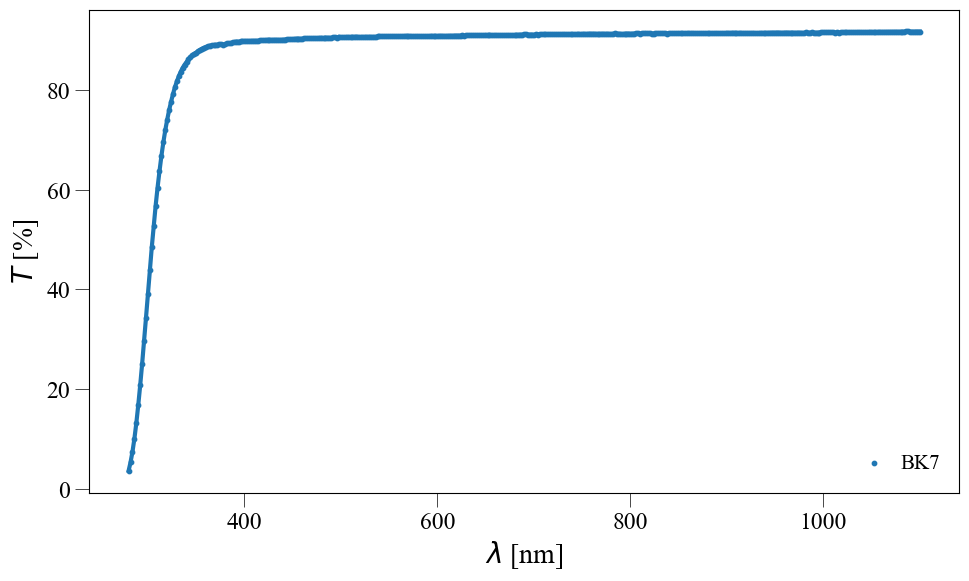
\includegraphics[scale=0.35]{bk7_1}
                \captionsetup{justification=centering, font=footnotesize}
                \captionof{figure}{Závislost propustnosti na vlnové délce pro sklo BK7.}
                \label{fig:bk7_1}
                \raggedright
                \vspace{10pt}   
                \par \centering
                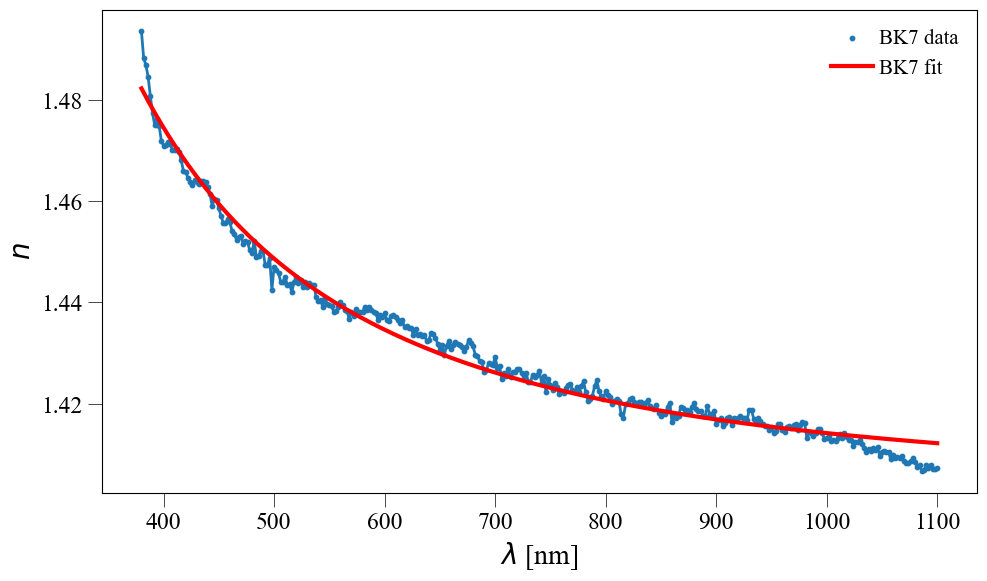
\includegraphics[scale=0.35]{bk7_2}
                \captionsetup{justification=centering, font=footnotesize}
                \captionof{figure}{Závislost indexu lomu na vlnové délce pro sklo BK7.}
                \label{fig:bk7_2}
                \vspace{10pt}
                \raggedright
                Dále jsme změřili propustnost pro červený filtr s nominální propustností 663 nm. Výsledky měření jsou uvedeny v grafu (4). 
                \par Z grafu je patrné, že maximum propustnosti se vyskytuje na vlnové délce: 
                \begin{center}
                    $\lambda_{max}$ = 670(2) nm
                \end{center}
                \vspace{10pt}   
                \par \centering
                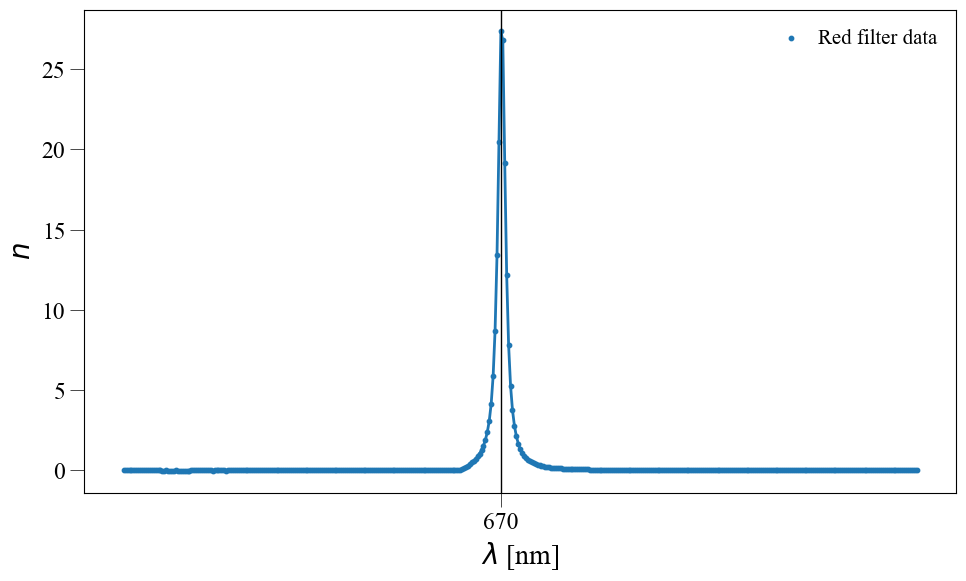
\includegraphics[scale=0.35]{red}
                \captionsetup{justification=centering, font=footnotesize}
                \captionof{figure}{Závislost propustnosti na vlnové délce pro červený filtr.}
                \label{fig:red}
                \vspace{10pt}
                \raggedright
                Poté jsme pro určení tloušťky desky TiO$_2$ změřili propustnost skla SiO$_2$ a skla SiO$_2$ s příměsí TiO$_2$. Naměřené údaje jsou uvedeny v grafu (5) a v tabulce (3).
    \end{minipage}
\newpage
    \begin{minipage}[t]{0.5\textwidth}
                \vspace{-15pt}   
                \par \centering
                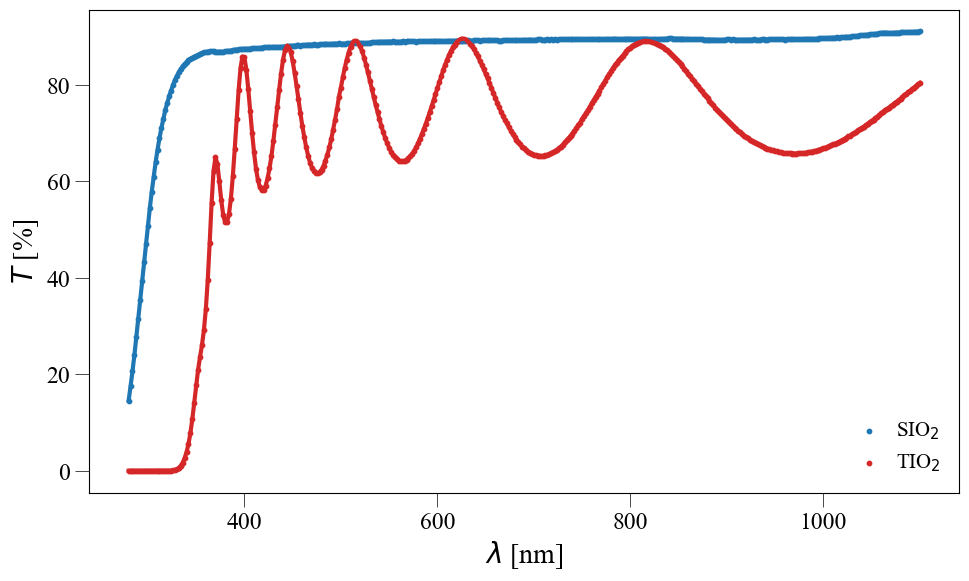
\includegraphics[scale=0.35]{sklo}
                \captionsetup{justification=centering, font=footnotesize}
                \captionof{figure}{Závislost propustnosti na vlnové délce pro sklo SiO$_2$ a sklo SiO$_2$ s příměsí TiO$_2$.}
                \label{fig:sklo}
                \vspace{10pt}
                \raggedright
                \par Pomocí vzorců (4), (8), (7), (6) a (5) byly vypočteny hodnoty $n_s$, $R_s$, $T_m$, $T^{min}_f$ a $n_{\nu}$ pro minima propustnosti skla s příměsí TiO2. Tyto výpočty jsou uvedeny v tabulce (1).
                \par Odtud byla vypočtena tloušťka materiálu pro pět párů minimálních vlnových délek podle vzorce (9): 
                \vspace{10pt}
                \par \centering
                \begin{tabular}{|c|c|c|c|c|}
                    \hline
                    $\lambda$ [nm] & $\lambda'$ [nm] & n & n$'$ & d [nm] \\
                    \hline
                    420 & 474 & 2.9639 & 2.7652 & 408.71(5) \\
                    \hline
                    474 & 564 & 2.7652 & 2.6453 & 437.31(5) \\
                    \hline
                    564 & 706 & 2.6453 & 2.5943 & 492.31(6) \\
                    \hline
                    706 & 968 & 2.5943 & 2.5706 & 490.60(6) \\
                    \hline
                \end{tabular}
                \captionsetup{justification=centering, font=footnotesize}
                \captionof{table}{Výpočet tloušťky materiálu pro pět párů minimálních vlnových délek.}
                \vspace{20pt}
                \raggedright
                Odtud získáme hodnotu tloušťky desky: 
                \begin{center}
                    $d$ = (457$\pm$100) nm
                \end{center}
            \subsection{Lambert-Beerův zákon}   
                Dále jsme změřili propustnost čtyř desek se stejným materiálem. Destičky byly do spektrometru vkládány jedna po druhé, takže na konci jsme měli vrstvu čtyř destiček, které se vzájemně překrývaly. Výsledky měření jsou uvedeny v grafu (6).
                \par Předpokládá se, že tloušťka desek $d$ je stejná. Po měření byla získána následující hodnota $d$: 
                \begin{center}
                    $d$ = 3.51(2) mm
                \end{center}
    \end{minipage}
    \hspace{10pt}  
    \begin{minipage}[t]{0.5\textwidth} 
                \vspace{-15pt}   
                \par \centering
                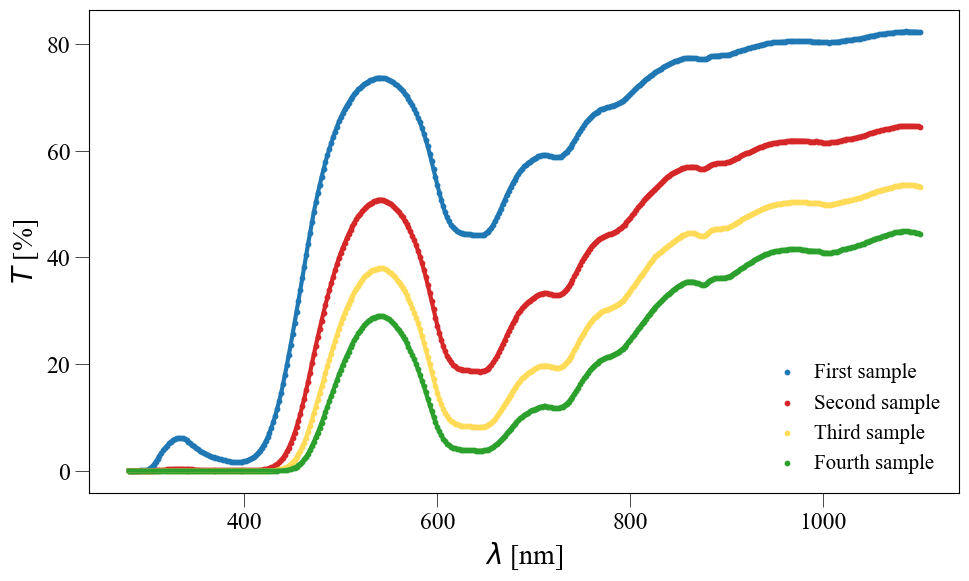
\includegraphics[scale=0.35]{alam}
                \captionsetup{justification=centering, font=footnotesize}
                \captionof{figure}{Závislost propustnosti vrstev desky na vlnové délce.}
                \label{fig:alam}
                \vspace{10pt}
                \raggedright
                \par Poté jsme vypočítali hodnoty $ln(T)$ čtyř různých kombinací destiček ve spektrografu pro čtyři pevné vlnové délky. Poté jsme je vynesli do grafu závislosti $ln(T)$ na tloušťce vrstvy desky $d$. Poté jsme pro potvrzení platnosti vzorce (10) data lineárně aproximovali a získali tak hodnotu absorpčního koeficientu $\alpha$. 
                \par Výsledky jsou uvedeny v tabulce (2) a na obrázku (7).
                \vspace{10pt}
                \par \centering
                \begin{tabular}{|c|c|c|c|c|c|}
                    \hline
                    \multicolumn{1}{|c}{} & \multicolumn{4}{|c|}{$ln(T)$ [\%]} &  \\
                    \hline
                    $\lambda$ [nm] & 3.51 & 7.02 & 10.53 & 14.04 & $\alpha$ [m$^{-1}$] \\
                    \hline
                    500 & -0.411 & -0.894 & -1.285 & -1.662 & 118(5) \\
                    \hline
                    600 & -0.624 & -1.301 & -1.923 & -2.503 & 178(4) \\
                    \hline
                    700 & -0.536 & -1.126 & -1.661 & -2.166 & 155(4) \\
                    \hline
                    800 & -0.347 & -0.746 & -1.089 & -1.405 & 100(4) \\
                    \hline
                    900 & -0.248 & -0.548 & -0.787 & -1.014 & 72(3) \\
                    \hline
                \end{tabular}
                \captionsetup{justification=centering, font=footnotesize}
                \captionof{table}{Výpočet absorpčního koeficientu $\alpha$ pro čtyři pevné vlnové délky a čtyři různé tloušťky vrstvy desky.}
                \vspace{10pt}
                \raggedright 
                \par \centering
                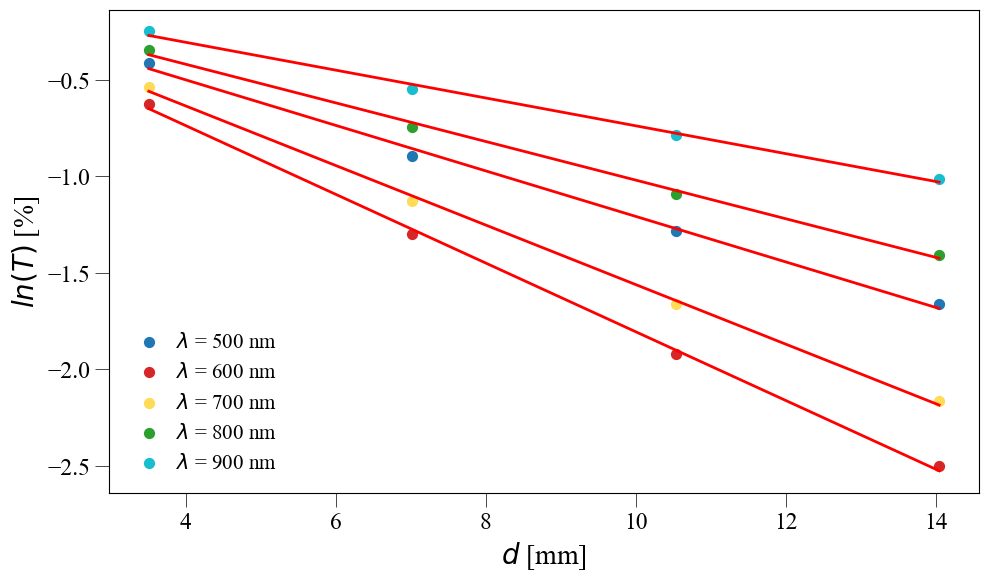
\includegraphics[scale=0.35]{ln}
                \captionsetup{justification=centering, font=footnotesize}
                \captionof{figure}{Závislost $ln(T)$ na tloušťce vrstvy desky $d$.}
                \label{fig:ln}
                \vspace{10pt}
                \raggedright
    \end{minipage}
                \vspace{15pt}
                \par \centering
                \begin{tabular}{|c|c|c|c|c|c|c|c|}
                    \hline
                    $\lambda$ [nm] &  $T_{ss, SiO_2}$ [\%]  & $T_{fs, TiO_2}$ [\%] & $n_s$ & $R_s$ & $T_m$ [\%] & $T^{min}_f$ [\%] & $n_{\nu}$ \\
                    \hline
                    420 & 87.8 & 58.3 & 1.4027(2) & 0.02809(3) & 66.4 & 63.951(2) & 2.9639(4) \\
                    \hline
                    474 & 88.4 & 61.7 & 1.4027(2) & 0.02809(3) & 69.9 & 67.318(2) & 2.7652(3) \\
                    \hline
                    564 & 89.0 & 64.2 & 1.4027(2) & 0.02809(3) & 72.1 & 69.499(2) & 2.6453(3) \\
                    \hline
                    706 & 89.4 & 65.3 & 1.4027(2) & 0.02809(3) & 73.0 & 70.464(2) & 2.5943(3) \\
                    \hline
                    968 & 89.5 & 65.8 & 1.4027(2) & 0.02809(3) & 73.5 & 70.920(2) & 2.5706(3) \\
                    \hline
                \end{tabular}
                \captionsetup{justification=centering, font=footnotesize}
                \captionof{table}{Výpočet veličin pro minima propustnosti skla s příměsí TiO2.}
                \vspace{20pt}
                \raggedright
\newpage
    \begin{minipage}[t]{0.5\textwidth} 
                \par Ze vzorce (10) pak zjistíme hodnoty $\alpha$ pro všechny naměřené vlnové délky každé desky. Výsledky měření jsou patrné z grafu (8).
                \vspace{10pt}
                \raggedright 
                \par \centering
                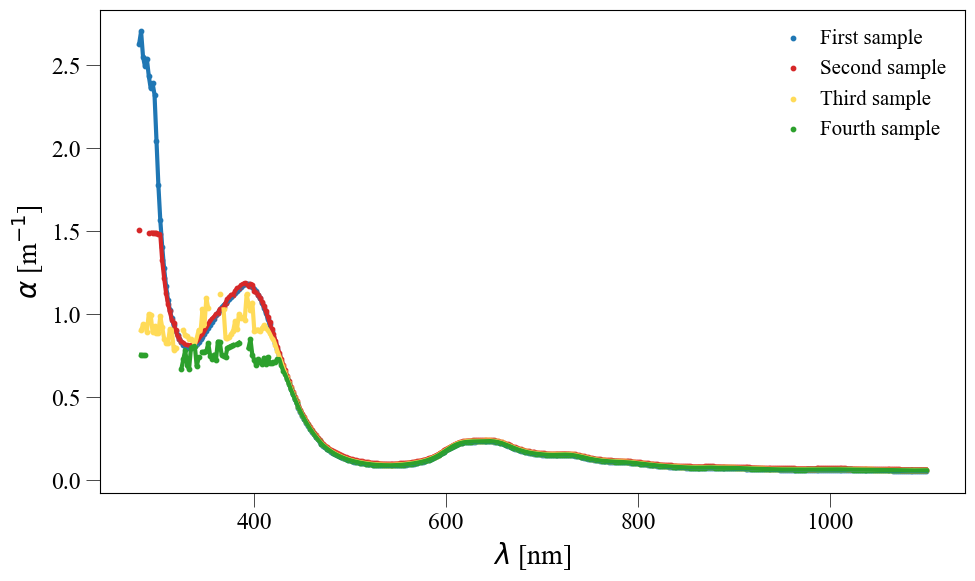
\includegraphics[scale=0.35]{alpha}
                \captionsetup{justification=centering, font=footnotesize}
                \captionof{figure}{Závislost absorpčního koeficientu $\alpha$ na vlnové délce.}
                \label{fig:alpha}
                \vspace{10pt}
                \raggedright
                \par Z tohoto grafu je patrné, že Lambertův-Beerův zákon platí v intervalu vlnových délek $\lambda \in$ [400,1000] nm.
                \vspace{10pt}
                \par K výpočtu veličin a jejich nejistot byla použita knihovna Uncertinties pro Python: \href{pypi.org/project/uncertainties}. Kód je přiložen k protokolu. 
        \section{Závěr}  
            \subsection{Měření spektrální propustnosti}
                Byla změřena spektrální závislost propustnosti skla BK7. Byla získána hodnota indexu lomu $n$ v závislosti na vlnové délce $\lambda$, $A$ = $n_0$ = 1.4027(2) a $B$ = 1.149(7)$\times$10$^4$ nm$^2$. 
                \par Byla změřena propustnost červeného filtru s nominální propustností 663 nm. Byla získána hodnota maximální propustnosti $\lambda_{max}$ = 670(2) nm.
                \par Byla změřena propustnost skla SiO$_2$ a skla SiO$_2$ s příměsí TiO$_2$. Byla získána hodnota tloušťky desky $d$ = (457$\pm$100) nm.
            \subsection{Lambert-Beerův zákon}
                Byla změřena závislost propustnosti vrstev desky na vlnové délce. Byla získána hodnota tloušťky desky $d$ = 3.51(2) mm.
                \par Byl stanoven interval platnosti Lambertova-Beerova zákona $\lambda \in$ [400,1000] nm.
    \end{minipage}
    \hspace{10pt}
    \begin{minipage}[t]{0.5\textwidth} 
    \end{minipage}
\newpage
    \par K výpočtu chyb byl použit následující kód: 
    \begin{lstlisting}[language=Python, basicstyle=\tiny, breaklines=true, postbreak=\mbox{\textbackslashspace}]
        #Importing the libraries

        import matplotlib.pyplot as plt
        import numpy as np
        import pandas as pd
        from scipy import stats
        from scipy.stats import t as t 
        from scipy.optimize import curve_fit
        from uncertainties import *
        from uncertainties.umath import *
        
        #Reading data

        BK7 = pd.read_csv('data/BK7.csv')
        ALAM1 = pd.read_csv('data/ALAM1.csv')
        ALAM2 = pd.read_csv('data/ALAM2.csv')
        ALAM3 = pd.read_csv('data/ALAM3.csv')
        ALAM4 = pd.read_csv('data/ALAM4.csv')
        RED = pd.read_csv('data/663_RED.csv')
        SIO2 = pd.read_csv('data/SIO2.csv')
        TIO2 = pd.read_csv('data/TIO2.csv')
        out = pd.read_excel('data/out.xlsx')

        # Constants and values

        I_0 = 280 

        def uncert(data_input, uncert_inst):
        t_coeff = t.ppf((1 + 0.99)/2, len(data_input)-1)
        return np.sqrt((np.std(data_input)/np.sqrt(len(data_input)))**2 + uncert_inst**2)*t_coeff

        #Canculations for BK7

        BK7['T'] = BK7['T']

        BK7['n'] = (1 + np.sqrt(1 - (BK7['T']/100))) / (BK7['T']/100)

        # Define the polynomial function

        def polynomial_fit(values, A, B):
            return A + B / (values**2)

        # Use curve_fit to find the parameters A and B
        initial_guess = [1.5, 40000]  # Initial guess for parameters A and B
        params, covariance = curve_fit(polynomial_fit, BK7['lambda'][50:], BK7['n'][50:], p0=initial_guess)

        # Extract the optimized parameters
        A_optimized, B_optimized = params
        A_error, B_error = np.sqrt(np.diag(covariance))

        A_comb = ufloat(A_optimized, A_error)
        B_comb = ufloat(B_optimized, B_error)

        # Print the optimized parameters
        print('A =', A_comb)
        print('B =', B_comb)

        #Best-fit line

        n_val = polynomial_fit(BK7['lambda'][50:], A_optimized, B_optimized)

        # Calculation 

        out['lambda'] = SIO2['lambda']
        out['T_sio2'] = SIO2['T']
        out['T_tio2'] = TIO2['T']
        out['n_sio2'] = (1 + np.sqrt(1 - (SIO2['T']/100))) / (SIO2['T']/100)
        R_sio2 = (A_comb-1)**2 / (A_comb+1)**2
        out['T_m'] = out['T_tio2'] / out['T_sio2']
        out['T_min'] = out['T_m'] * (1-R_sio2)/(1+R_sio2*(1-out['T_m']))

        n_v_list = []
        for ii,ID in enumerate(out['T_min']):
            n_v_list.append(((1+sqrt(1-out['T_min'][ii]))/(out['T_min'][ii])) * sqrt(A_comb))
        out['n_v'] = n_v_list

        print('\nR_sio2 =', R_sio2)

        # print(out.iloc[51])
        # print(f'\n{out.iloc[70]}')
        # print(f'\n{out.iloc[97]}')
        # print(f'\n{out.iloc[142]}')
        # print(f'\n{out.iloc[213]}')
        # print(f'\n{out.iloc[344]}')

        lambda_list = [out.iloc[70]['lambda'], out.iloc[97]['lambda'], out.iloc[142]['lambda'], out.iloc[213]['lambda'], out.iloc[344]['lambda']]
        n_v_list = [out.iloc[70]['n_v'], out.iloc[97]['n_v'], out.iloc[142]['n_v'], out.iloc[213]['n_v'], out.iloc[344]['n_v']]

        d_list = []
        for ii,ID in enumerate(lambda_list):
            if ii == len(lambda_list)-1:
                break
            d_list.append((lambda_list[ii]*lambda_list[ii+1])/(2*(n_v_list[ii]*lambda_list[ii+1]-n_v_list[ii+1]*lambda_list[ii])))

        print(f'\n{d_list}')

        d_nominal_values = [item.nominal_value for item in d_list]
        d_std_devs = [item.std_dev for item in d_list]
        d = ufloat(np.mean(d_nominal_values), uncert(d_nominal_values, np.mean(d_std_devs)))

        print('\nd =', d.nominal_value, '+-', d.std_dev)

        d_2 = ufloat(3.51, 0.02)
        d_list_2 = [3.51, 7.02, 10.53, 14.04]
        d_2_list = [500,600,700,800,900]
        ln_500 = []
        ln_600 = []
        ln_700 = []
        ln_800 = []
        ln_900 = []

        for ii,ID in enumerate(ALAM1['lambda']):
            if ID == 500.0000305:
                ln_500.append(np.log(ALAM1['T'][ii]/100))
                ln_500.append(np.log(ALAM2['T'][ii]/100))
                ln_500.append(np.log(ALAM3['T'][ii]/100))
                ln_500.append(np.log(ALAM4['T'][ii]/100))
            elif ID == 600.0000000:
                ln_600.append(np.log(ALAM1['T'][ii]/100))
                ln_600.append(np.log(ALAM2['T'][ii]/100))
                ln_600.append(np.log(ALAM3['T'][ii]/100))
                ln_600.append(np.log(ALAM4['T'][ii]/100))
            elif ID == 700.0000610:
                ln_700.append(np.log(ALAM1['T'][ii]/100))
                ln_700.append(np.log(ALAM2['T'][ii]/100))
                ln_700.append(np.log(ALAM3['T'][ii]/100))
                ln_700.append(np.log(ALAM4['T'][ii]/100))
            elif ID == 800.0000610:
                ln_800.append(np.log(ALAM1['T'][ii]/100))
                ln_800.append(np.log(ALAM2['T'][ii]/100))
                ln_800.append(np.log(ALAM3['T'][ii]/100))
                ln_800.append(np.log(ALAM4['T'][ii]/100))
            elif ID == 900.0000610:
                ln_900.append(np.log(ALAM1['T'][ii]/100))
                ln_900.append(np.log(ALAM2['T'][ii]/100))
                ln_900.append(np.log(ALAM3['T'][ii]/100))
                ln_900.append(np.log(ALAM4['T'][ii]/100))

        ln_list = [ln_500, ln_600, ln_700, ln_800, ln_900]

        ALAM1['alpha'] = - np.log(ALAM1['T']/100) / d_list_2[0]
        ALAM2['alpha'] = - np.log(ALAM2['T']/100) / d_list_2[1]
        ALAM3['alpha'] = - np.log(ALAM3['T']/100) / d_list_2[2]
        ALAM4['alpha'] = - np.log(ALAM4['T']/100) / d_list_2[3]

        # print(out)

        # Linear regression

        #Calculate linear regression

        fit_line_list = []

        for ii,ID in enumerate(ln_list):

            slope, intercept, r_value, p_value, std_err = stats.linregress(d_list_2, ID)

            alpha = ufloat(slope, std_err)
            print(f'alpha({ii}) =', alpha*(-1000))

            #Best fit line 
            best_fit_line = slope * np.array(d_list_2) + intercept

            fit_line_list.append(best_fit_line)
    \end{lstlisting}
\end{document}